% Author: Dominik Harmim <xharmi00@stud.fit.vutbr.cz>
% Author: Vojtěch Hertl <xhertl04@stud.fit.vutbr.cz>


\documentclass[a4paper, 11pt]{article}


\usepackage[czech]{babel}
\usepackage[utf8]{inputenc}
\usepackage[left=2cm, top=3cm, text={17cm, 24cm}]{geometry}
\usepackage{times}
\usepackage{graphicx}
\usepackage[unicode]{hyperref}
\hypersetup{
	colorlinks = true,
	hypertexnames = false,
	citecolor = red
}


\begin{document}
	%%%%%%%%%%%%%%%%%%%%%%%%%%%%%%%% Titulní stránka %%%%%%%%%%%%%%%%%%%%%%%%%%%
	\begin{titlepage}
		\begin{center}
			
\includegraphics[width=0.77\linewidth]{inc/FIT_logo.pdf} \\

			\vspace{\stretch{0.382}}

			\Huge{Simulační studie} \\
			\LARGE{\textbf{Rozvoz jídla firmou Freshbox}} \\
			\Large{Tým: ModelX} \\
			\Large{Varianta 2: Doprava zboží nebo osob}

			\vspace{\stretch{0.618}}
		\end{center}

		\begin{minipage}{0.5 \textwidth}
			{\Large \today}
		\end{minipage}
		\hfill
		\begin{minipage}[r]{0.5 \textwidth}
			\Large
			\begin{tabular}{l l}
				\textbf{Dominik Harmim} & \textbf{(xharmi00)} \\
				Vojtěch Hertl & (xhertl04) \\
			\end{tabular}
		\end{minipage}
	\end{titlepage}



	%%%%%%%%%%%%%%%%%%%%%%%%%%%%%%%% Obsah %%%%%%%%%%%%%%%%%%%%%%%%%%%%%%%%%%%%%
	\pagenumbering{roman}
	\setcounter{page}{1}
	\tableofcontents
	\clearpage



	%%%%%%%%%%%%%%%%%%%%%%%%%%%%%%%% Úvod %%%%%%%%%%%%%%%%%%%%%%%%%%%%%%%%%%%%%%
	\pagenumbering{arabic}
	\setcounter{page}{1}

	\section{Úvod}

	V~této práci je řešen proces sestavování modelu \cite[snímek 7]{IMS_slides}
	pro rozvoz jídla po Brně firmou Freshbox \cite{Freshbox} a~jeho následná
	simulace \cite[snímek 33]{IMS_slides}. Díky tomuto modelu a~simulačním
	experimentům \cite[snímek 9]{Freshbox} nad ním je možno pozorovat
	efektivitu a~přínos v~různých podmínkách. Smyslem experimentů je zjistit,
	jak kvalitně navržený je systém \cite[snímek 18]{IMS_slides} a~zda by se
	změnou některého z~ovlivňujících faktorů mohl zdokonalit.


	\subsection{Autoři, zdroje}

	Projekt vypracovali studenti Dominik Harmim a~Vojtěch Hertl z~FIT VUT
	v~Brně.

	K~technické části této práce bylo využito zdrojů z~kursu Modelování
	a~simulace na FIT VUT v~Brně. Jako zdroj k~faktům sloužily webové stránky
	firmy Freshbox a~také vedoucí této firmy, Mgr. Silvie Obadalová\\
	(\texttt{obadalova@freshbox.cz}).


	\subsection{Ověření validity}

	Ověřování validity \cite[snímek 37]{Freshbox} probíhalo telefonicky
	a~elektronicky s~vedoucí firmy Freshox, magistrou Obadalovou. Na základě
	této komunikace byla získána všechna data potřebná k~experimentálnímu
	ověřování validity modelu. Validita byla také ověřena pomocí experimentů
	a~srovnáním s~realitou.



	%%%%%%%%%%%%%%%% Rozbor tématu a použitých metod/technologií %%%%%%%%%%%%%%%
	\section{Rozbor tématu a~použitých metod/technologií}

	Všechna použitá fakta jsou zprůměrována ze všech získaných informací. \\

	Zákazníci mají předem objednaná jidla od firmy Freshbox, která tato jídla
	každý den od 6:30 hod. do 12:30 hod. rozváží zákazníkům po Brně a~okolí.
	Firma Freshbox rozváží jidlo A auty, přičemž jedno auto
	je schopné naložit  maximálně B jídel. Každý den se rozváží
	průměrně C jídel. Firma má na začátku rozvozu již všechna jídla
	připravena a~v~6:30 se připraví všechna auta, do kterých se naloží
	maximální počet jídel, který je dán kapacitou auta. Naložení jednoho
	auta průměrně trvá D minut. Rozvoz všech jídel jednoho auta
	trvá průměrně E minut. Při tomto rozvozu každé auto urazí
	průměrně F km. Pro rozvoz se požívají auta značky Volkswagen Caddy TDI.
	Tato auta mají spotřebu H l/100km banzínu/nafty. Když auto rozveze
	všechna naložená jídla, vrátí se na pobočku Freshbox, aby se mohla
	naložit další jídla. Tento proces se opakuje tak dlouho, dokud nejsou
	rozvezena všechna jídla. Jeden zákazník (právnická nebo fyzická osoba)
	si samozřejmě může objednat více jídel na jedno místo doručení.
	Průměrná hodnota objednávky jednoho zákazníka v~jeden den činí I Kč.


	\subsection{Použité postupy}

	Pro vytvoření modelu byl použit programovací jazyk C++ za podpory
	simulační knihovny SIMLIB \cite{SIMLIB}. Tyto technologie jsou ideální pro
	řešení zadaného problému, jelikož poskytují všechna potřebná rozhraní
	k~implementaci modelu. Dále byly použity postupy popsané v textech
	ke kursu Modelování a simulace na FIT VUT v~Brně \cite{IMS_slides}
	k~vytváření Petriho sítě \cite[snímek 123]{IMS_slides} a~samotnému
	programování za použití knihovny SIMLIB.


	\subsection{Popis původu použitých metod/technologií}

	TODO vyjmenovat všechny technologie a autory u nich, např.
	Knihovna SIMLIB ve verzi ..., autor Dr. Ing. Petr Peringer.
	-- až nakonec, až budu vědět, co všechno se použilo



	%%%%%%%%%%%%%%%%%%%%%%%%%%%%%%%% Koncepce modelu %%%%%%%%%%%%%%%%%%%%%%%%%%%
	\section{Koncepce modelu}

	V~této sekci se zpracovává návrh konceptuálního modelu[TODO] nad
	systémem, který je brán jako systém hromadné obsluhy. Při vytváření
	je potřeba vybrat ze všech údajů ty podstatné informace pro model. Jak lze
	vyčíst z~rozboru tématu, důležité je, namodelovat všecho, co souvisí
	se samotným rozvozem. Díky skutečnosti, že časové údaje jsou průměry
	zjištěných časů, je zřejmé, že bude dostatečné simulovat průběh
	jednoho dne, přičemž se samozřejmě může den ode dne nepatrně lišit.
	Na všechny časové údaje při modelování se tedy použije rovnoměrné
	rozdělení[TODO] s~určitým rozptylem. Aby se model zjednodušil,
	průměrný počet jídel, který se každý den rozváží, se zaokrouhlí,
	aby byl dělitelný maximální kapacitou aut. Na validitu to má nepatrný
	vliv, dá se říci, že zanedbatelný. Dále značka auta, spotřeba paliva
	a~cena nejsou pro model důležitá, tyto informace budou použity při
	zefektivňování systému. Přesto, že tato situace reálně často nenastává,
	pro lepší experimentování je přidán druhý koncový stav, který znamená,
	že směna skončí dříve než jsou rozvezena všechna jídla, tedy nějaká
	jídla zbydou na skladě. Předpokládá se také, že auto, které započne
	ještě během pracovní směny svůj cyklus, ho celý dokončí.


	\subsection{Popis konceptuálního modelu}

	Model se skládá ze~dvou hlavních větví. První značí samotný průběh
	rozvozu jídel a~druhá časovač. Druhá z~větví jen určuje, jak dlouho
	probíhá pracovní směna, to je 6 hodin, a~jakmile směna skončí, skončí
	rozvoz jídel. První větev má dvě vstupní proměnné - počet aut a~počet
	jídel. Auto zde slouží jako obslužná linka, kde pokud je některé volné
	a~připravené na rozvoz a~zároveň jsou ještě nějaká jídla na skladě,
	začnou se nakládat. Pokud je však některé z~aut připraveno na rozvoz,
	ale již byla všechna jídla rozvezena, skončí pracovní směna. Po
	naložení jídel se auto vydá na cestu a všechna jídla rozveze. Po ukončení
	této činnosti je auto zase volné a~připraveno k použití.


	\subsection{Forma konceptuálního modelu}

	Model je vizualizován pomocí Petriho sítě[TODO] v~příloze
	\ref{appendix:petri_net}.



	%%%%%%%%%%%%%%%%%%% Architektura simulačního modelu %%%%%%%%%%%%%%%%%%%%%%%%
	\section{Architektura simulačního modelu}


	\subsection{Mapování konceptuálního modulu do simulačního modelu}



	%%%%%%%%%%%%%%% Podstata simulačních experimentů a jejich průběh %%%%%%%%%%%
	\section{Podstata simulačních experimentů a~jejich průběh}


	\subsection{Postup experimentování}


	\subsection{Experimenty}


	\subsection{Závěry experimentů}



	%%%%%%%%%%%%%%%%% Shrnutí simulačních experimentů a závěr %%%%%%%%%%%%%%%%%%
	\section{Shrnutí simulačních experimentů a~závěr}



	%%%%%%%%%%%%%%%%%%%%%%%%%%%%%%%% Citace %%%%%%%%%%%%%%%%%%%%%%%%%%%%%%%%%%%%
	\clearpage
	\bibliographystyle{czechiso}
	\renewcommand{\refname}{Literatura}
	\bibliography{documentation}



	%%%%%%%%%%%%%%%%%%%%%%%%%%%%%%%% Přílohy %%%%%%%%%%%%%%%%%%%%%%%%%%%%%%%%%%%
	\clearpage
	\appendix

	\section{Petriho síť}
	\label{appendix:petri_net}
	\begin{figure}[!ht]
		\centering
		\vspace{-1.2cm}
		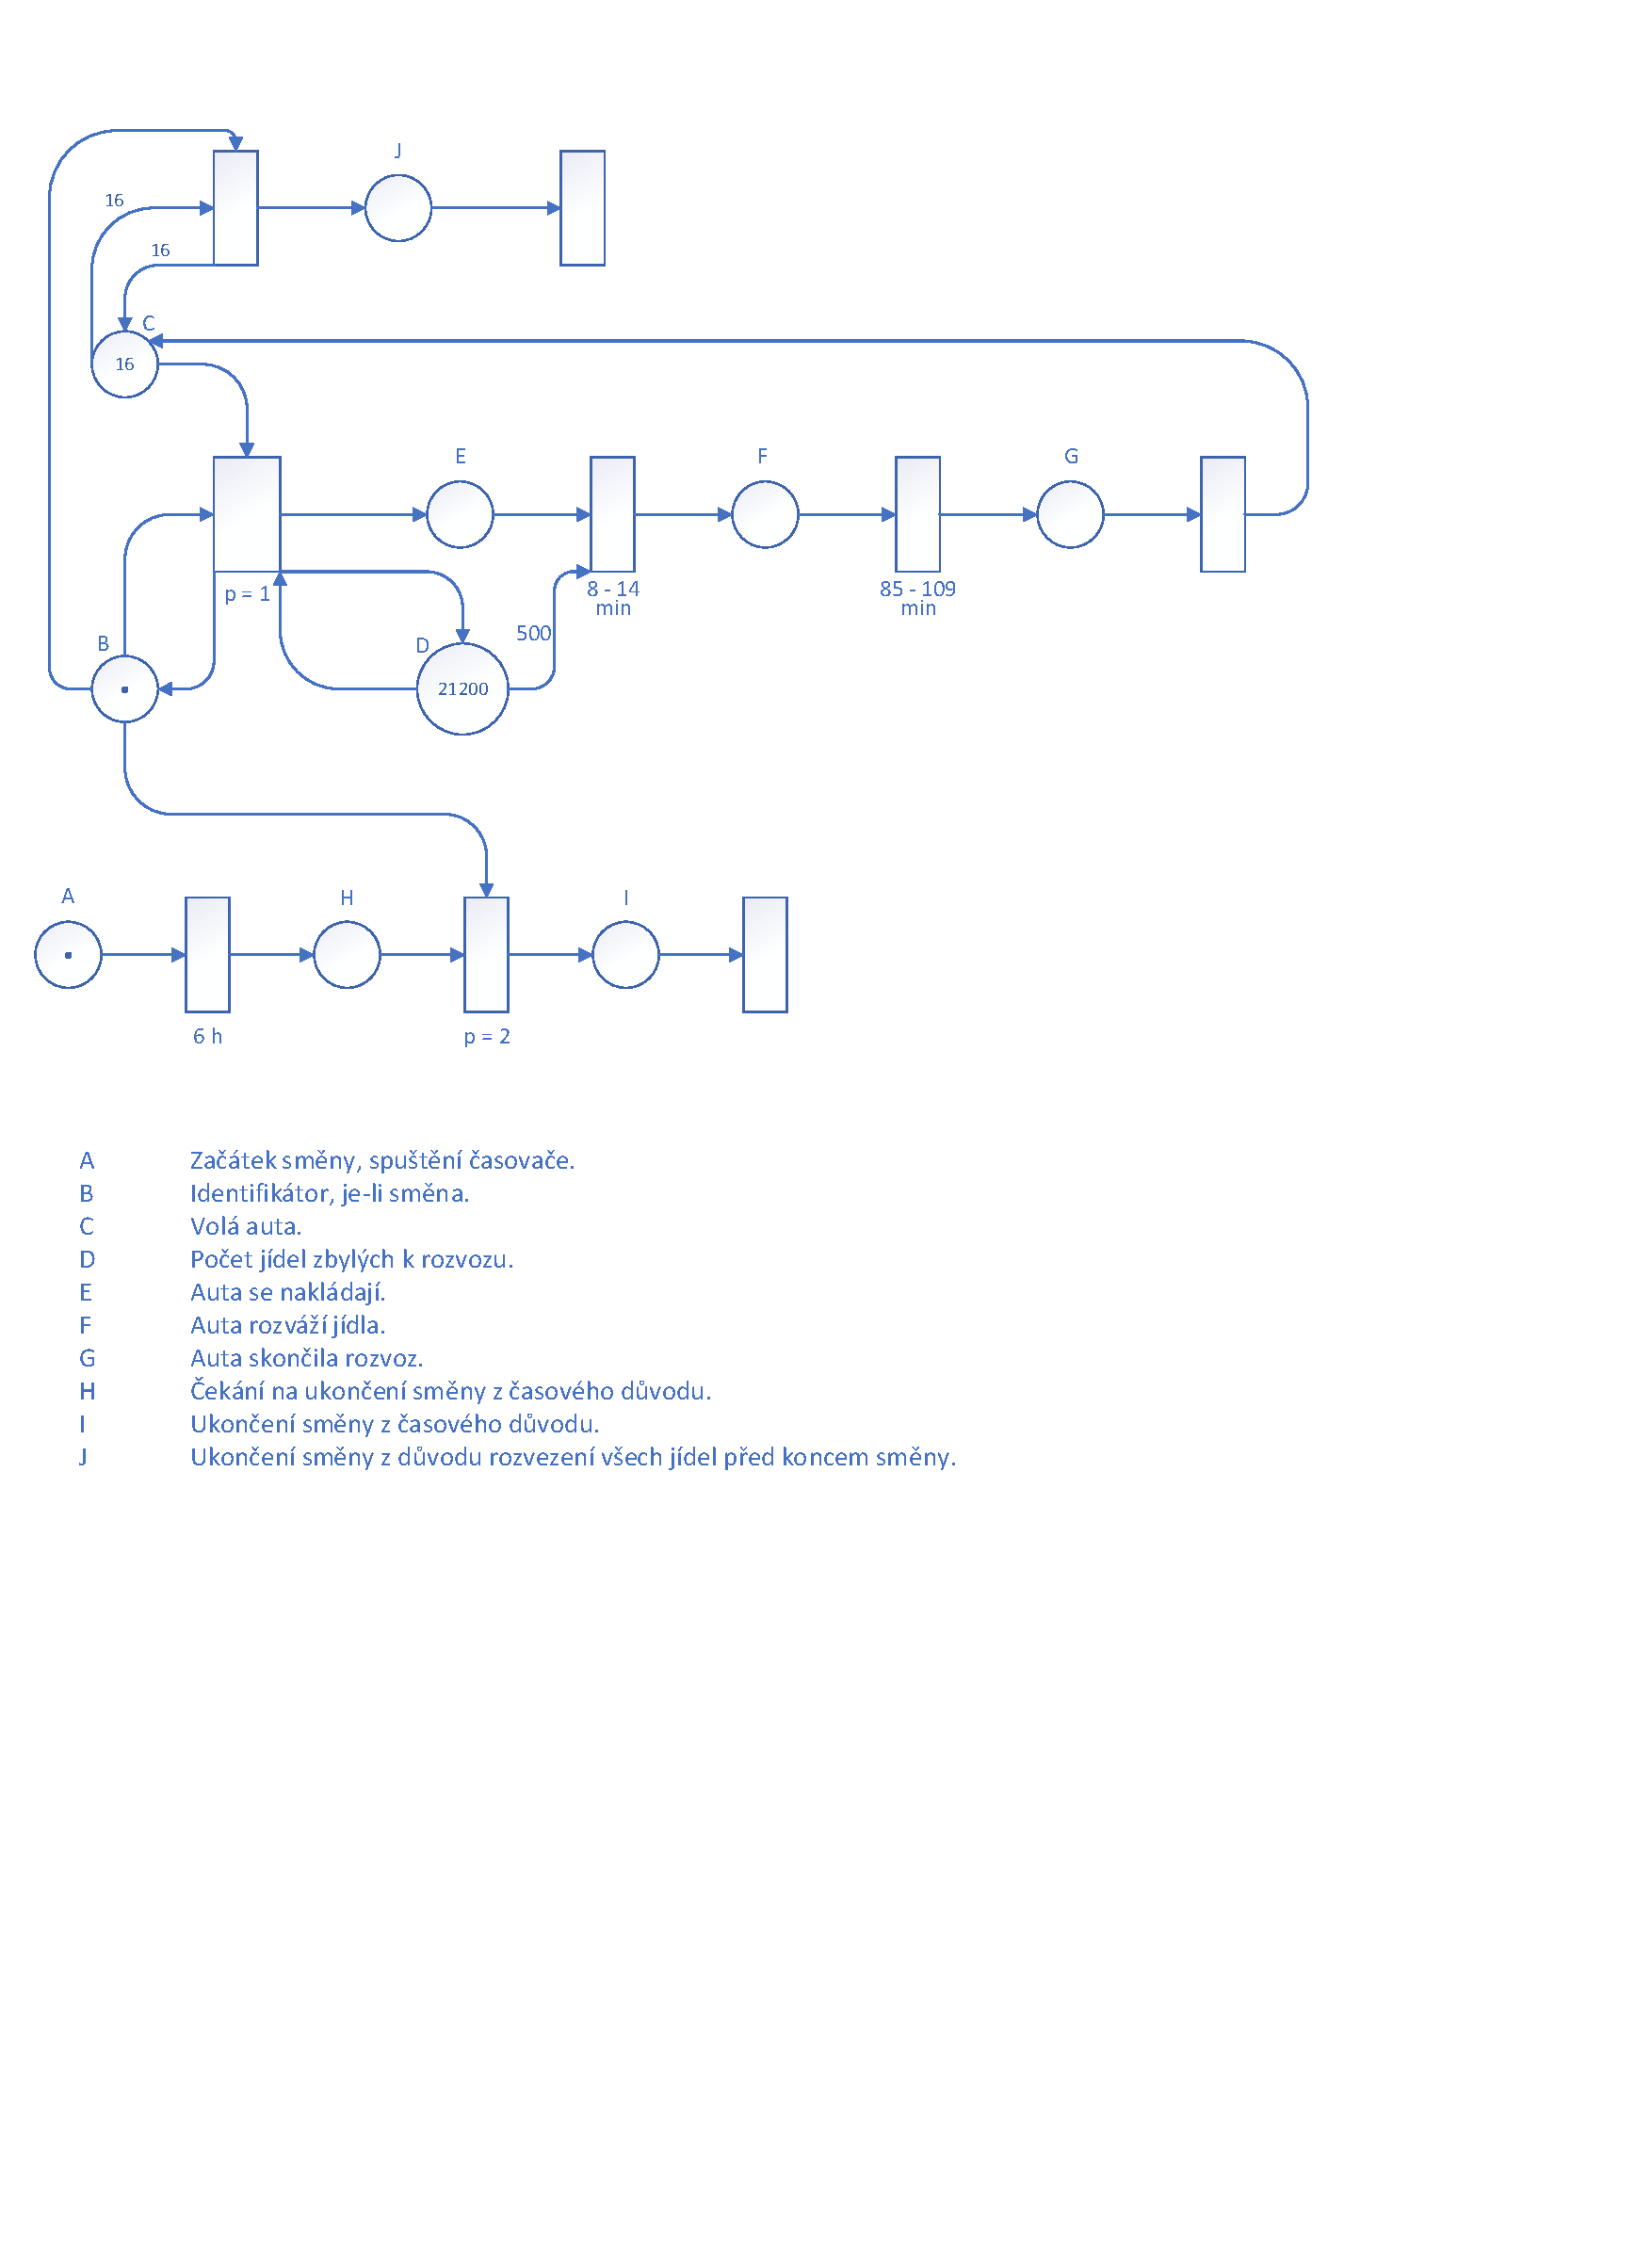
\includegraphics[width=0.95\linewidth]{inc/petri_net.pdf}
		\caption{Petriho síť}
		\label{figure:petri_net}
	\end{figure}
\end{document}
